
\documentclass[11pt]{article}

\usepackage{alltt,epsfig,amsmath,amssymb}
\usepackage{fullpage} % one inch margins

\usepackage{graphicx}
\graphicspath{ {images/} }

% inline code
\def\code#1{\texttt{#1}}
% block code
\usepackage{listings}
\lstset{
  numbers=none,
  showstringspaces=false,
  frame=L,
  language=c++,
  xleftmargin=\parindent,
  breaklines=true,
  keepspaces=true
  basicstyle=\ttfamily,
}

% block quotes
\usepackage{csquotes}

\usepackage{fancyhdr}
\fancypagestyle{plain}{
  \fancyhf{}% Clear header/footer
  \fancyhead[L]{}
  \fancyfoot[C]{\thepage}
  \fancyhead[R]{C++ Functional Collections}
  \setlength{\headsep}{0.2in}
}

\pagestyle{plain}   % Set page style to plain.

\author{Ian Zapolsky, Nate Brennand and Uday Singh}
\title{Functional Collections in C++}


\begin{document}
\setlength{\parskip}{.1 in}

\maketitle
\newpage

\section{Introduction}


Collections are fundamental to most programming tasks because they allow the user to group and process large sets of data.
However, when it comes to expressing moderately complex collection manipulations, C++ is markedly behind some of its more modern counterparts with respect to code clarity and efficiency of space.
This is the problem we set out to solve.

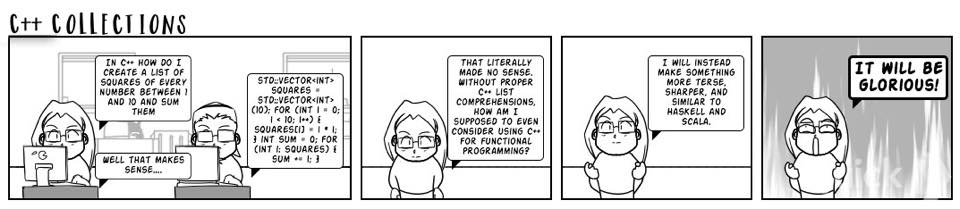
\includegraphics[width=\textwidth]{comic}


Languages are used as tools to communicate, and consequently, the structure and limitations of the languages we use determine the way we think.
This idea, known in the field of linguistic relativity as the Sapir-Whorf hypothesis\cite{linguistic_relativity}, has critical implications when applied to programming languages, namely that the ability of a programmer to reason about a problem can be limited by the languages he or she has learned (or has yet to learn).
Furthermore, if we hold this hypothesis to be true, we can reasonably conclude that learning how to write code in a new language can provide a programmer with a totally new way of thinking about solving a problem that he or she may have already solved a dozen times before.

C++ is an interesting language in this respect because in recent years it has begun to introduce new language constructs that help it blur the lines between programming paradigms along which programming languages are usually divided.
Perhaps most notably, C++11 introduced a set of features that allows for functional programming in the language.
Functional programming is a programming paradigm that avoids state and favors immutable variables.
It is as if the English language introduced a new group of words, whose meanings were all missing from the original dictionary.
The conclusion we are tempted to draw from this addition is that C++ is a great language to learn, because its new functional vocabulary will allow the programmer who learns it to think about problems both from a traditional C++ perspective, and now also from a functional perspective.

Unfortunately, the ease of use of many of C++'s functional features pales in comparison to that of other functional languages, making it daunting for beginners in functional programming to use the features correctly, if at all.

\blockquote{In 24 hours you might be able to learn some of the syntax of C++ (if you already know another language), but you couldn't learn much about how to use the language. In short, if you were, say, a Basic programmer, you could learn to write programs in the style of Basic using C++ syntax, but you couldn't learn what C++ is actually good (and bad) for. So what's the point? Alan Perlis once said: "A language that doesn't affect the way you think about programming, is not worth knowing" -- Peter Norvig\cite{norvig}
}

C++ Collections is a library built on top of C++11 that provides both finite and infinite collections data structures, built from the ground up with syntax in mind.
It strives to make functional programming concepts, specifically to do with lists, more accessible and understandable to C++ programmers.

An additional perk of functional languages is the terseness associated with them.
Software bugs per line of code have been found to be constant across different languages\cite{code_complete} which indicates that more succint operations on lists are more likely to operate as intended.

To use the C++ Collections library, download it from Github and simply \code{\#include cpp\_collections.h} in your source file.



\section{Collections}

C++ Collections provides traditional, functional abstractions on lists.

The Collection class is used to represent any finite list.

Assume you would like to create a list of numbers from 1 to 100, sum them, and then store the value in an \code{int}.
The Collection class allows you to achieve this in one line of code.

\begin{lstlisting}
int sum = range(1, 101).reduceLeft([](int x, int y) {
    return x + y;});
\end{lstlisting}

Note the similarity to the syntax provided by functional languages like Haskell and Scala.

\begin{lstlisting}[language=haskell]
sum = foldl1 (+) [1..100]
\end{lstlisting}

\begin{lstlisting}
val sum = Range(1, 101).reduce((a,b) => a+b)
\end{lstlisting}

\subsection{Implementation Details}

The Collection class uses the heavily optimized \code{std::vector} to store data internally.
Consequently, Collections are very fast and reliable.
They are also fully type-generic and can be efficiently constructed from a variety of existing STL data structures, including vectors, lists, arrays, and C-style arrays.
What differentiates the Collection from the \code{std::vector} is mainly the functions defined on top of it, such as \code{map}, \code{zip}, \code{reduce}, and \code{fold}.
Despite the movement of modern C++ toward functional programming, these traditional functional methods are generally absent from the language.
If they are present, they exist as generalized STL functions, not member functions of existing data structures (see \code{std::accumulate}).




\section{Streams}

The Stream class is used to represent potentially infinite lists of data.
This is a fairly common concept in functional programming languages but is rare in C++.
Streams can be converted to finite Collections via the \code{take()} function.

Observe the following example, again computing the sum of the numbers 1 to 100.

\begin{lstlisting}
Stream<int> ints = from(1);
Collection<int> ints_1_100 = ints.take(100);
int sum = ints_1_100.reduceLeft([](int x, int y) {return x + y;});
\end{lstlisting}

...or...

\begin{lstlisting}
int sum = from(1).take(100).reduceLeft([](int x, int y) {return x + y;});
\end{lstlisting}

Here, we define the infinite Stream with the \code{from()} function, which by default returns a Stream of elements of its argument's type where each element is incremented by 1.
We then use the \code{take()} function to convert our Stream into a finite Collection.
We then reduce this Collection with an addition function.

Note that Streams can be arbitrarily complex.
Below, we define a Stream to generate the Fibonacci sequence with the help of one of the Stream creation functions provided by the C++ Collections library.


\begin{lstlisting}
auto fibs = recurrence([](std::tuple<int,int> t) {
    return std::get<0>(t) + std::get<1>(t);
}, std::make_tuple(0, 1));

std::cout << fibs.take(5) << std::endl;
// [0,1,1,2,3]
\end{lstlisting}





\subsection{Implementation Details}

The Stream class is a self-referential data structure, meaning that in addition to the head, or the first value in the list, the class stores a pointer to a function that returns another Stream at all times.
Recall the definition of the Fibonacci Stream generator from above.
Written without the macro, the definition is as follows:

\begin{lstlisting}
std::function<Stream<int>(int, int)> fibs = [&](int prev, int curr) -> Stream<int> {
    return Stream<int>(curr, [=]() -> Stream<int> {
        return fibs(curr, prev + curr);
    });
};

Stream<int> tenfibs = fibs(0, 1).take(3);
\end{lstlisting}

The Stream generator \code{fibs}, when called with arguments \code{0} and \code{1}, creates a new Stream that has a head value of 1 and an internal pointer to the function `fibs(1, 1)`.
Then, when we ask to \code{take(3)} elements from the Stream, the structure returns its head, and then lazily computes the remainder of the elements it needs to satisfy our request.
It does this by returning the result of its stored function pointer.
In this case, `tenfibs` would first return 1 becuase that is its head.
It would then return the head of the Stream that results from the evaluation of the function it stores a pointer to, namely \code{fibs(1, 1)}, which is 1.
The result of \code{fibs(1, 1)} also stores a pointer to another function, \code{fibs(1, 2)}.
To find the third and final value, the Stream will evaluate this function and return the resulting Stream's head, which is 2.
For a step-by-step visual depiction of the underlying state of our Stream during the \code{take(3)} function call, see the graphic below:

\begin{lstlisting}
tenfibs.head      tenfibs.gen
     1             fibs(0,1)
     1             fibs(1,1)
     2             fibs(1,2)
     3             fibs(2,3)
\end{lstlisting}



\section{Pipelines}


The Collection and Stream classes are exciting because they allow C++ developers to construct complex pipelines of functions.
These functions consist of of three main types:

\begin{enumerate}
  \item{Source operators: methods that instantiate or create a Collection or Stream.}
  \item{Intermediate operators: methods that take a Collection or Stream as input and output a new Collection or Stream.}
  \item{Terminal operators: methods that take a Collection or Stream as input and output something that is not another Collection or Stream.}
\end{enumerate}

Pipelines can be formed by combining a source operator, one or more intermediate operators, and a terminal operator.
For example, summing the squares from 1 to 100 can be easily represented by the following pipeline:

\begin{lstlisting}
int sum = range(1, 101).map([](int x) { return x * x; }).reduceLeft([](int x, int y) { return x+y; });
\end{lstlisting}

Here, \code{range} is the source operator, \code{map} is an intermediate operator, and \code{reduceLeft} is a terminal operator.
Note how these pipelines can become arbitrarily complex by adding more intermediate operators.



\section{Collections Methods}


\subsection{Member Functions}


\subsubsection{\code{Collection<T>()}}

Construct an empty Collection.

\begin{lstlisting}[title=example]
auto empty_collection = Collection<int>();
\end{lstlisting}




\subsubsection{\code{Collection<T>(int size)}}

Construct a pre-sized Collection.

\begin{lstlisting}[title=example]
auto presized_collection = Collection<int>(5);
\end{lstlisting}




\subsubsection{\code{Collection<T>(std::vector<T> list)}}

Construct a Collection from a \code{std::vector}.

\begin{lstlisting}[title=example]
auto vector_collection = Collection<int>(std::vector<int> {1, 2, 3});
\end{lstlisting}




\subsubsection{\code{Collection<T>(std::list<T> list)}}

Construct a Collection from a \code{std::list}.

\begin{lstlisting}[title=example]
auto list_collection = Collection<int>(std::list<int> {1, 2, 3});
\end{lstlisting}





\subsubsection{\code{Collection<T>(std::array<T, size> list)}}

Construct a Collection from a \code{std::array}.

\begin{lstlisting}[title=example]
auto array_collection = Collection<int>(std::array<int,3> {1, 2, 3});
\end{lstlisting}




\subsubsection{\code{Collection<T>(T d[], int len)}}

Construct a Collection from a C-style array (requires length).

\begin{lstlisting}[title=example]
int int_c_array[] {1, 2, 3};
auto c_array_collection = Collection<int>(int_c_array, 3);
\end{lstlisting}




\subsubsection{\code{Collection<T>::vector()}}

Returns the Collection as a \code{std::vector}.




\subsubsection{\code{Collection<T>::list()}}

Returns the Collection as a \code{std::list}.




\subsubsection{\code{Collection<T>::size()}}

Returns an \code{int} with the current size of the Collection.




\subsubsection{\code{Collection<T>::head()}}

Returns the first element in the Collection.

\begin{lstlisting}[title=example]
auto a = range(1, 10);
std::cout << a.head(); << std::endl;

# 1
\end{lstlisting}




\subsubsection{\code{Collection<T>::last()}}

Returns the last element in the Collection.

\begin{lstlisting}[title=example]
auto a = range(1, 10);
std::cout << a.last(); << std::endl;

# 9
\end{lstlisting}




\subsubsection{\code{Collection<T>::init()}}

Return all elements except the last.

\begin{lstlisting}[title=example]
auto a = range(5);
std::cout << a.init() << std::endl;

# [0,1,2,3]
\end{lstlisting}




\subsubsection{\code{Collection<T>::tail()}}

Return all elements except the head.

\begin{lstlisting}[title=example]
auto a = range(5);
std::cout << a.tail() << std::endl;

# [1,2,3,4]
\end{lstlisting}




\subsubsection{\code{Collection<T>::pop\_head()}}

Remove the head of the collection.

\begin{lstlisting}[title=example]
auto a = range(5);
a.pop_head();
std::cout << a << std::endl;

# [1,2,3,4]
\end{lstlisting}




\subsubsection{\code{Collection<T>::each(std::function<void(T)> func)}}

Apply a function to all the elements in the Collection

\begin{lstlisting}[title=example]
int sum = 0;
auto a = range(5);
a.each([&](int x) {
    sum += x;
});
std::cout << sum << std::endl;

# 10
\end{lstlisting}




\subsubsection{\code{Collection<T>::filter(std::function<bool(T)> func)}}

Return a subset of the Collection containing the elements of the original Collection that pass a predicate function.

\begin{lstlisting}[title=example]
auto a = range(1,11);
std::cout << a.filter([](int x) { return x % 2 == 0; }) << std::endl;

# [2,4,6,8,10]
\end{lstlisting}




\subsubsection{\code{Collection<T>::slice(int low, int high)}}

Return the elements whose indices are within the range \code{[low, high)}.

\begin{lstlisting}[title=example]
auto a = range(10, 20);
std::cout << a.slice(1,4) << std::endl;

# [11,12,13]
\end{lstlisting}





\subsubsection{\code{Collection<T>::map(Function func)}}

Return the Collection that results from the transformation of each element in the original Collection.

\begin{lstlisting}[title=example]
auto a = range(3);
std::cout << a.map([](int x) { return x+1; }) << std::endl;

# [1,2,3]
\end{lstlisting}




\subsubsection{\code{Collection<T>::tmap(Function func, int threads)}}

An alternative implementation of map that uses multiple concurrent
std::threads to speed up processing.

\begin{lstlisting}[title=example]
auto a = range(3);
std::cout << a.tmap([](int x) { return x+1; }, 3) << std::endl;

# [1,2,3]
\end{lstlisting}





\subsubsection{\code{Collection<T>::reduceLeft(std::function<T(T, T)> func)}}

Return the result of the application of the same binary operator on adjacent pairs of elements in the Collection, starting from the left.

\begin{lstlisting}[title=example]
int sum = range(5).reduceLeft([](int x, int y) { return x+y; });
std::cout << sum << std::endl;

# 10
\end{lstlisting}




\subsubsection{\code{Collection<T>::reduceRight(std::function<T(T, T)> func)}}

Return the result of the application of the same binary operator on adjacent pairs of elements in the Collection, starting from the right.





\subsubsection{\code{Collection<T>::treduce(std::function<T(T, T)> func, int threads)}}

An alternative implementation of reduce that uses multiple concurrent threads to speed up processing
(note that the function passed to treduce must be commutative to achieve accurate result).

\begin{lstlisting}[title=example]
int sum = range(5).treduce([](int x, int y) { return x+y; }, 3);
std::cout << sum << std::endl;

# 10
\end{lstlisting}




\subsubsection{\code{Collection<T>::foldLeft(Function func, U init)}}

Return the result of the application of the same binary operator on all elements in the Collection as well as an initial value, starting from the left.

\begin{lstlisting}[title=example]
int sum = range(5).foldLeft([](int x, int y) { return x+y; }, 0);
std::cout << sum << std::endl;

# 10
\end{lstlisting}




\subsubsection{\code{Collection<T>::foldRight(Function func, U init)}}

Return the result of the application of the same binary operator on all elements in the Collection as well as an initial value, starting from the right.




\subsubsection{\code{Collection<T>::scanLeft(Function func, U init)}}

Returns the intermediate results of the binary accumulation of the elements in a Collection as well as an initial value, starting from the left.

\begin{lstlisting}[title=example]
auto ints = range(1,5);
auto ints2 = ints.scanLeft([](int x, int y) { return x+y; }, 1);
std::cout << ints2 << std::endl;

# [1,2,4,7,11]
\end{lstlisting}




\subsubsection{\code{Collection<T>::scanRight(Function func, U init)}}

Returns the intermediate results of the binary accumulation of the elements in a Collection as well as an initial value, starting from the left.

\begin{lstlisting}[title=example]
auto ints = range(1,5);
auto ints2 = ints.scanRight([](int x, int y) { return x+y; }, 1);
std::cout << ints2 << std::endl;

# [11,10,8,5,1]
\end{lstlisting}




\subsection{Non-member Functions}

\subsubsection{\code{concat()}}

Return the Collection that results from the concatentation of an arbitrary number of Collections of the same type.

\begin{lstlisting}[title=example]
auto a = range(3);
auto b = range(3);
auto c = range(3);
std::cout << concat(a, b, c) << std::endl;

# [0,1,2,0,1,2,0,1,2]
\end{lstlisting}





\subsubsection{\code{range(T size)}}

Return Collection of numeric types over the range \code{[0, size)}.

\begin{lstlisting}[title=example]
auto a = range(5);
std::cout << a << std::endl;

# [0,1,2,3,4]
\end{lstlisting}




\subsubsection{range(T low, T high)}

Return Collection of numeric types over the range \code{[low, high)}.

\begin{lstlisting}[title=example]
auto a = range(5, 10);
std::cout << a << std::endl;

# [5,6,7,8,9]
\end{lstlisting}





\subsubsection{zip(Collection<U>... other)}

Return a Collection of tuples, where each tuple contains the elements of the zipped Collections that occur at the same position.

\begin{lstlisting}[title=example]
auto a = range(3);
auto b = range(3.0);
auto c = Collection(std::vector<char> {'a','b','c'});

auto d = zip(a, b, c);

assert(d[0] == std::make_tuple(0, 0.0, 'a'));
\end{lstlisting}




\subsubsection{zipWith(Function func, Collection<U>... other)}
Generalizes \code{zip} by zipping with the function given as the first argument instead of a tupling function.

\begin{lstlisting}[title=example]
auto a = range(3);
auto b = range(3);
std::cout << zipWith([](int x, int y) { return x+y; }, a, b) << std::endl;

# [0,2,4]
\end{lstlisting}




\section{Stream Methods}

\subsection{Member Functions}

\subsubsection{\code{Stream<T>(T head, std::function<T>()> gen)}}

Default Stream constructor.
Takes an initial head value, and a function that returns a Stream.
The programmer should not have to interact with this method directly.
Instead, use the one of the four Stream creation helper functions, \code{from()}, \code{repeat()}, \code{iterate()}, or \code{recurrence()}.


\begin{lstlisting}[title=example]
std::function<Stream<int>()> ones = [&]() { return Stream<int>(1, ones) };
std::cout << ones().take(3) << std::endl;

// [1,1,1]
\end{lstlisting}

\subsubsection{\code{Stream<T>(T head, Stream<T> tail)}}

Tail-only Stream constructor.
The programmer should not have to interact with this method directly.

\subsubsection{\code{Stream<T>::head()}}

Return the first element of the Stream.

\begin{lstlisting}[title=example]
std::cout << from(1).head() << std::endl;

// 1
\end{lstlisting}

\subsubsection{\code{Stream<T>::tail()}}

Return the Stream minus the current head.

\begin{lstlisting}[title=example]
std::cout << from(1).tail().head() << std::endl;

// 2
\end{lstlisting}

\subsubsection{\code{Stream<T>::take(int n)}}

Return \code{n} elements taken from the Stream as a Collection.

\begin{lstlisting}[title=example]
std::cout << from(1).take(5) << std::endl;

// [1,2,3,4,5]
\end{lstlisting}

\subsubsection{\code{Stream<T>::filter(std::function<bool(T)> func)}}

Return a Stream that contains the elements of the initial Stream that match the predicate function.

\begin{lstlisting}[title=example]
auto evens = from(1).filter([](int x) { return x % 2 == 0; });
std::cout << evens.take(5) << std::endl;

// [2,4,6,8,10]
\end{lstlisting}

\subsubsection{\code{Stream<T>::map(Function func)}}

Return the Stream that results from the transformation of each element in the original Stream.

\begin{lstlisting}[title=example]
auto squares = from(1).map([](int x) { return x * x; });
std::cout << squares.take(5) << std::endl;

// [1,4,9,16,25]
\end{lstlisting}

\subsection{Non-member Functions}

\subsubsection{\code{cons(T value, Stream<T> other)}}

Prepends a value to a Stream.

\begin{lstlisting}[title=example]
auto ints = from(1);
std:cout << cons(10, ints).take(5) << std::endl;

// [10,1,2,3,4]
\end{lstlisting}

\subsubsection{\code{operator\&(T value, Stream<T> other)}}

Prepends a value to a Stream.

\begin{lstlisting}[title=example]
auto ints = from(1);
std:cout << (10 & (20 & ints)).take(5) << std::endl;

// [10,20,1,2,3]
\end{lstlisting}

\subsubsection{\code{repeate(T value)}}

Construct an infinite Stream of the given value.

\begin{lstlisting}[title=example]
std:cout << repeat(1).take(5) << std::endl;

// [1,1,1,1,1]
\end{lstlisting}


\subsubsection{\code{from(T n, T step=1)}}

Construct a Stream, starting at n, incrementing by step (defaults to 1).

\begin{lstlisting}[title=example]
std:cout << from(1).take(5) << std::endl;

// [1,2,3,4,5]
\end{lstlisting}

\subsubsection{\code{iterate(T value, Function func)}}

Construct an infinite Stream in terms of an initial value \code{x}, and a function \code{f}.
The Stream is then constructed as \code{x, f(x), f(f(x)), f(f(f(x)))...}.

\begin{lstlisting}[title=example]
std::cout <<  iterate(0, [](int x) { return x+1; }).take(5) << std::endl;

// [0,1,2,3,4]
\end{lstlisting}

\subsubsection{\code{recurrence(Function func, std::tuple<U...> args)}}

A generalized version of \code{iterate()}, which allows the user to define an infinite Stream in terms of any number of arguments, stored in a tuple, and a function that takes that tuple.

\begin{lstlisting}[title=example]
auto fibs = recurrence([](std::tuple<int,int> t) {
    return std::get<0>(t) + std::get<1>(t);
}, std::make_tuple(0, 1));
std::cout << fibs.take(5) << std::endl;

// [0,1,1,2,3]
\end{lstlisting}



\subsubsection{\code{zip(Stream<U>... other)}}

Return a Stream of tuples, where each tuple contains the elements of the zipped Streams that occur at the same position

\subsubsection{\code{zipWith(Function func, Stream<U>... other)}}

Generalizes zip by zipping with the function given as the first argument instead of a tupling function.





\section{Development Support}
If you are interested in contributing, please fork our repository and submit a pull request on Github \cite{github}.

\section{Testing}


The test suite is composed of tests to check that we stop all errors at the compilation stage, not at runtime.
Files placed in the \code{tests/} directory will be compiled against \code{collections.h}.

Files with \code{fail\_} at the start of the filename will be expected to fail.

Those without will be expected to build.
Buildable files will also be executed.
They should include assertions to insure the library is executing as desired.
Passing tests should not include any output to stdout/stderr.


Executable with \code{make}:

\begin{lstlisting}
make test
\end{lstlisting}




\subsection{Subsets}

A subset of the tests can be run by utilizing the \code{run\_tests.sh} script directly.
If an argument is provided, only the tests matching it will be run.

\begin{lstlisting}[title=Ex. Run all tests matching reduce]
./run_tests.sh reduce
\end{lstlisting}






% citations
\bibliographystyle{abbrv}
\bibliography{bibliography}

\end{document}

